% Adjust these for the path of the theme and its graphics, relative to this file
%\usepackage{beamerthemeFalmouthGamesAcademy}
\usepackage{../../beamerthemeFalmouthGamesAcademy}
\usepackage{multimedia}
\graphicspath{ {../../} }

% Default language for code listings
\lstset{language=Python,
        morekeywords={each,in,nullptr}
}

% For strikethrough effect
\usepackage[normalem]{ulem}
\usepackage{wasysym}

\usepackage{pdfpages}

% //www.texample.net/tikz/examples/state-machine/
\usetikzlibrary{arrows,automata}

\newcommand{\modulecode}{COMP260}\newcommand{\moduletitle}{Distributed Systems}\newcommand{\sessionnumber}{5}

\setbeamertemplate{navigation symbols}{}

\newcommand{\fullbleed}[1]{
\begin{frame}[plain]
	\begin{tikzpicture}[remember picture, overlay]
		\node[at=(current page.center)] {
			\includegraphics[width=\paperwidth]{#1}
		};
	\end{tikzpicture}
\end{frame}
}

\newcommand{\picturepage}[2]{
\begin{frame}[plain]
	\begin{tikzpicture}[remember picture, overlay]
		\node[at=(current page.center)] {
			\includegraphics[width=\paperwidth]{#1}
		};
		\draw<1>[draw=none, fill=black, opacity=0.9] (-1,-5.2) rectangle (current page.south east);
		\node[draw=none,text width=0.96\paperwidth, align=right] at (5.5,-5.5) {\tiny{#2}};
	\end{tikzpicture}
\end{frame}
}

\newcommand{\notepicx}[5]{
\begin{frame}[plain]
	\begin{tikzpicture}[remember picture, overlay]
		\node[at=(current page.center)] {
			\includegraphics[width=\paperwidth]{#1}
		};
		\node[draw=none, fill=black, text width=#5\paperwidth] at ([xshift=#3, yshift=#4] current page.center) {\small{#2}};
	\end{tikzpicture}
\end{frame}
}

\newcommand{\notepic}[4]{
	\notepicx{#1}{#2}{#3}{#4}{0.4}
}

\begin{document}
\title{\sessionnumber: Tinkering Graphics I}
\subtitle{\modulecode: \moduletitle}

\frame{\titlepage} 

\begin{frame}
	\frametitle{Learning Outcomes}
	By the end of this workshop, you should be able to:	
	\begin{itemize}
		\item \textbf{Apply} knowledge of colour models to \textbf{write} code that manipulates pixels in a Visual Studio Form App
		\item \textbf{Use} functions, arguments, and basic data structures such as arrays
	\end{itemize}
\end{frame}

\begin{frame}
	\frametitle{Activity \#1a -- Setup}
	
	In pairs:
	
	\vspace{2em}
	
	\begin{itemize}		
		\item Open Visual Basic 
		\item Create a 'Windows Forms Application'
		\item Refer to the following documentation for details:
	\end{itemize}
\scriptsize \url{https://docs.microsoft.com/en-us/visualstudio/ide/create-csharp-winform-visual-studio}
\end{frame}

\begin{frame}[fragile]
	\frametitle{Activity \#1a -- Setup}
	
\begin{lstlisting}
int width = 640, height = 320;
Bitmap bmp = new Bitmap(width, height);

for (int y = 0; y < height; y++)
	{
	for (int x = 0; x < width; x++)
	{
		bmp.SetPixel(x, y, Color.FromArgb(255, 0, 0, 0));
	}
}
pictureBox1.Image = bmp;
bmp.Save("D:\\images\blackImage.png");
\end{lstlisting}
Note: This is an example that is contained in the 'Form' class
\end{frame}
\begin{frame}[fragile]
	\frametitle{Activity \#1a -- Setup}
	
Add a \textbf{Picturebox} from \textbf{Tools}. Set the \textbf{Picturebox} to \textbf{Zoom}.
NOTE - ADD SCREENSHOT TO ILLUSTRATE
\end{frame}

\begin{frame}
		\frametitle{Key C\# Methods Used}
			\begin{itemize}		
			\item \texttt{Bitmap} - consists of the pixel data for a graphics image and its attributes.
				\begin{itemize}	
					\item \texttt{New} - Initializes a new instance of the Bitmap class with the specified size or from an existing file.
					\item \texttt{Save} - Saves the Image to the specified file or stream.
				\end{itemize}	
			\item \texttt{SetPixel} - Sets the color of the specified pixel in a Bitmap.
			\item \texttt{GetPixel} - Gets the color of the specified pixel in a Bitmap.
			\item \texttt{Color.FromArgb} - Creates a colour structure from the four 8-bit ARGB components (alpha, red, green, and blue) values.	
			\end{itemize}
\end{frame}	

\begin{frame}[fragile]
	\frametitle{Key Concepts}
	
	\textbf{Nested} \texttt{for} \textbf{Loops} - to iterate through all the positions in a two dimensional array. For example: all the pixels in an image which are arranged in rows and columns.
	
	\begin{lstlisting}
for (int hours = 0; hours < 24; hours++)
{
	for (int minutes = 0; minutes < 60; minutes++)
	{
		//do something for every minute in the day
	}
}
	\end{lstlisting}
	
\end{frame}

\begin{frame}
	\frametitle{Activity \#1b -- Setup}
	
	In pairs:
	
	\vspace{2em}
	
	\begin{itemize}		
		\item Render a green \texttt{Bitmap} image
		\item Refer to the following documentation:
		\begin{itemize}
			\item \url{https://docs.microsoft.com/en-us/dotnet/api/system.drawing.color.fromargb}
			\item \url{https://docs.microsoft.com/en-us/dotnet/api/system.drawing.bitmap.setpixel}
		\end{itemize}
	\end{itemize}
\end{frame}

\begin{frame}[fragile]
	\frametitle{Activity \#2 - Test Card}

\begin{itemize}		
	\item Create a \texttt{Bitmap} image that displays 3 equal vertical bars of red, green and blue
	\item The image must be \textbf{640 x 480} in size.
	\item Consider how you will allocate the painting of pixels to the different areas of the screen. 

\end{itemize}
	
\center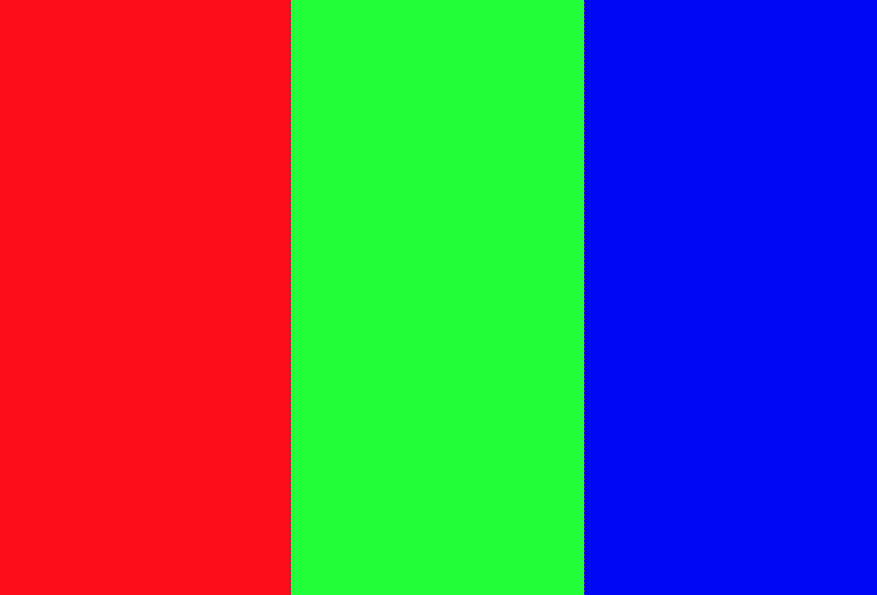
\includegraphics[scale=0.16]{testCard}

\end{frame}

\begin{frame}[fragile]
	\frametitle{Activity \#3 - Random Pixels}

\begin{itemize}		
	\item Create a \texttt{Bitmap} image that displays random pixel for every pixel in the image. Like snow on an old TV.
	\item Consider how you will generate random values for ARGB
	\item You will need to explore these methods associated with the \texttt{Random} class:
	
\end{itemize}
	
\begin{lstlisting}
 new Random();
\end{lstlisting}
Initializes a new instance of the \texttt{Random} class.
\begin{lstlisting}
Next();
\end{lstlisting}
Returns a non-negative random integer.

\end{frame}

\begin{frame}[fragile]
	\frametitle{Activity \#3 - Random Pixels}
\begin{columns}
	\begin{column}{0.48\textwidth}
	\begin{lstlisting}
Random rand = new Random();
	\end{lstlisting}
Create a variable to contain the \texttt{Random} class.
	\begin{lstlisting}
int a = rand.Next(256);
	\end{lstlisting}
Assign a variable for each colour channel and use \texttt{Next} with the new random variable to randomly choose a value.

\end{column}
 \begin{column}{0.48\textwidth}
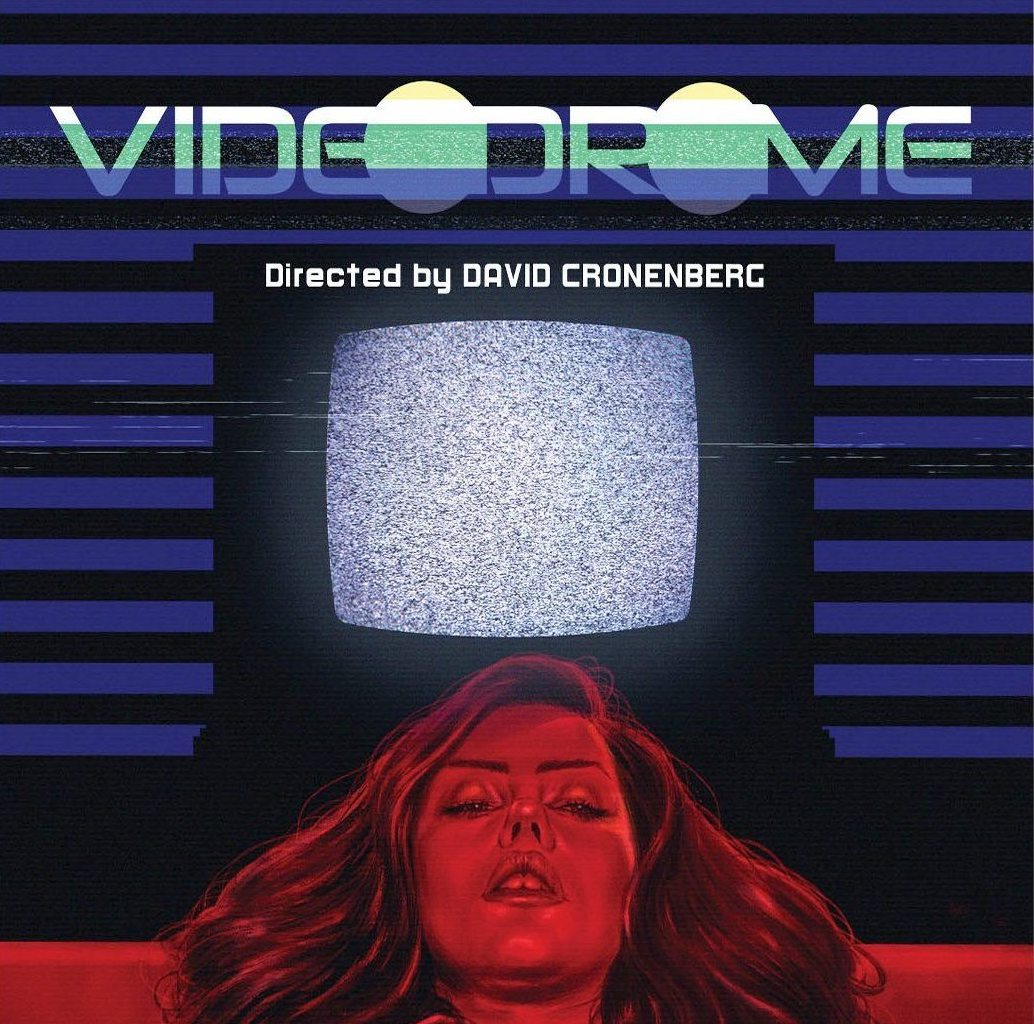
\includegraphics[scale=0.14]{videodrome}
\end{column}
\end{columns}
\end{frame}

\begin{frame}
	\frametitle{Activity \#2 -- Less Red}
	
	In pairs:
	
	\vspace{2em}
	
	\begin{itemize}		
		\item Define a function to load an image file to a \texttt{Surface}
		\item Then, define a function to reduce it's redness
		\item Refer to the following documentation:
		\begin{itemize}
			\item \url{https://www.pygame.org/docs/ref/image.html}
		\end{itemize}
	\end{itemize}
\end{frame}

\begin{frame}[fragile]
	\frametitle{Activity \#2 -- Less Red}

\begin{lstlisting}
my_surface = pygame.image.load('test.jpg')
\end{lstlisting}

\vspace{0.5em}

	
\begin{lstlisting}
def decreaseRed(pict):
  pixelMatrix = getPixels(pict)
  for pixel in pixelMatrix:
    value = getRed(pixel)
    setRedPixel(pixel, value * 0.5)
\end{lstlisting}

Note: Not all of this source code excerpt will work in PyGame.

\end{frame}

\begin{frame}
	\frametitle{Activity \#3 -- Swap Channel}
	
	In pairs:
	
	\vspace{2em}
	
	\begin{itemize}
		\item Define a function that turns all of the red values of pixels into blue values...
		\item ...and all of the blue values into red values
	\end{itemize}
\end{frame}

\begin{frame}[fragile]
	\frametitle{Activity \#3 -- Swap Channel}
	
\begin{lstlisting}
def swapRedBlueChannels(pict):
  pixelMatrix = getPixels(pict)
  for pixel in pixelMatrix:
    red_value = getRed(pixel)
    blue_value = getBlue(pixel)
    setRedPixel(pixel, blue_value)
    setBluePixel(pixel, red_value)
\end{lstlisting}

Note: This source code excerpt will not work in PyGame.

\end{frame}

\begin{frame}
	\frametitle{Activity \#4 -- Greyscale}
	
	In pairs:
	
	\vspace{2em}
	
	\begin{itemize}
		\item Define a function that loads an image and turns it to greyscale
		\item Consider the following calculation:
		\begin{itemize}
			\item $New Pixel Value = \frac{\Sigma Current Channel Value}{Number Of Channels}$
		\end{itemize}
	\end{itemize}
\end{frame}

\begin{frame}[fragile]
	\frametitle{Activity \#4 -- Greyscale}
	
\begin{lstlisting}
def loadGrayscale(file):
  pixelMatrix = getPixels(makePicture(file))
  for pixel in pixelMatrix:
    red = getRed(p)
    green = getGreen(p)
    blue = getBlue(p)
    
    pixelValue = (red+green+blue)/3
    
    setRedPixel(pixel,pixelValue)
    setGreenPixel(pixel, pixelValue)
    setBluePixel(pixel, pixelValue)
\end{lstlisting}

Note: This source code excerpt will not work in PyGame.

\end{frame}

\begin{frame}
	\frametitle{Activity \#5 -- Negative}
	
	In pairs:
	
	\vspace{2em}
	
	\begin{itemize}
		\item Define a function that loads an image and turns it to its negative
		\item Consider the following calculation:
		\begin{itemize}
			\item $New Channel Value = 255 - Current Channel Value$
		\end{itemize}
	\end{itemize}
\end{frame}

\begin{frame}[fragile]
	\frametitle{Activity \#5 -- Negative}
	
\begin{lstlisting}
def neg(picture):
  pixelMatrix = getPixels(makePicture(file))
  for pixel in pixelMatrix:
    red = getRed(p)
    green = getGreen(p)
    blue = getBlue(p)
        
    setRedPixel(pixel,255-red)
    setGreenPixel(pixel, 255-green)
    setBluePixel(pixel, 255-blue)
\end{lstlisting}

Note: This source code excerpt will not work in PyGame.

\end{frame}

\begin{frame}
	\frametitle{Activity \#6 -- Sunset}
	
	In pairs:
	
	\vspace{2em}
	
	\begin{itemize}
		\item Define a function that loads an image and produces several images as output, descreasing luminance
		\item Refer to the following documentation:
		\begin{itemize}
			\item \url{//www.pygame.org/docs/ref/time.html}
		\end{itemize}
	\end{itemize}
\end{frame}

\begin{frame}[fragile]
	\frametitle{Activity \#6 -- Sunset}

\begin{lstlisting}
def decreaseRed(picture, amount):
  for p in getPixels(picture):
    value=getRed(p)
    setRed(p,value*amount)

amount = 0.1 #tinker with this value
wait_time = 50 #tinker with this value    
    
for i in range(10):
  decreaseRed(picture, amount)
  decreaseGreen(picture, amount)
  decreaseBlue(picture, amount)
  wait(50)
\end{lstlisting}

Note: This source code excerpt will not work in PyGame.

\end{frame}

\begin{frame}
	\frametitle{Activity \#7 -- Top-Copy}
	
	In pairs:
	
	\vspace{2em}
	
	\begin{itemize}
		\item Define a function that copies the top half of a picture to its bottom half
		\item Refer to the following documentation:
		\begin{itemize}
			\item \url{https://docs.python.org/3.7/tutorial/introduction.html\#lists}
		\end{itemize}
	\end{itemize}
\end{frame}

\begin{frame}[fragile]
	\frametitle{Activity \#7 -- Top-Copy}

\begin{lstlisting}
def copyHalf(picture):
 pixels = getPixels(picture)
 for index in range(0,len(pixels)/2):
   sourcePixel = pixels[index]
   sourceRGBValue = getColor(sourcePixel)
   destinationPixel = pixels[index + len(pixels)/2]
   setColor(destinationPixel,sourceRGBValue)
 repaint(picture)
\end{lstlisting}

Note: This source code excerpt will not work in PyGame.

\end{frame}

\end{document}
